\chapter{自然数}
\section{你认为的自然数}
\paragraph{}自然数是如何被近代数学家构建?在一群杠精里,没点真本事是活不过一集。如果你没办法想象它如何严谨,那么我来告诉你。
\paragraph{}比如,我写了一个卖包子的程序,顾客来买包子,要几个包子程序就出几个包子。以严谨著称的升腾测试人员上场了:
\begin{tcolorbox}[storybox]
\begin{verse}
	\setlength{\leftmargini}{0em} % 取消左侧缩进
	\setlength{\baselineskip}{1.7em} 
	
	\textbf{她说:} 我要1千万个包子。 \\
	\textbf{程序:} 没有反应。(其实程序正在努力的做包子)\\
	\textbf{记下:} P2 bug, 很多包子买不了。\\
	\textbf{她说:} 2个包子,一个肉包,一个菜包。肉包里不要有肉,菜包里不要有菜。\\
	\textbf{程序:} 没有反应。(脑袋被门夹了)\\
	\textbf{记下:} P1 bug, 2个包子也买不了。\\
	\textbf{她说:} 给我来0个包子。\\
	\textbf{程序:} 崩溃。(不买就不买,凑什么热闹)\\
	\textbf{记下:} P0 bug,根本买不到包子。
\end{verse}
\end{tcolorbox}
\paragraph{}见识了上面测试人员的做法,就慢慢明白,为什么皮亚诺公理为什么要写得那么莫名其妙了。是的,做数学的人个个都是杠精,不整得无懈可击,会被抨得很惨。
\paragraph{}简单的说,如果让你来告诉我,什么是自然数,你会怎么告诉我?小朋友可能会说:先给我很多苹果,先有苹果然后才能数数。
\paragraph{}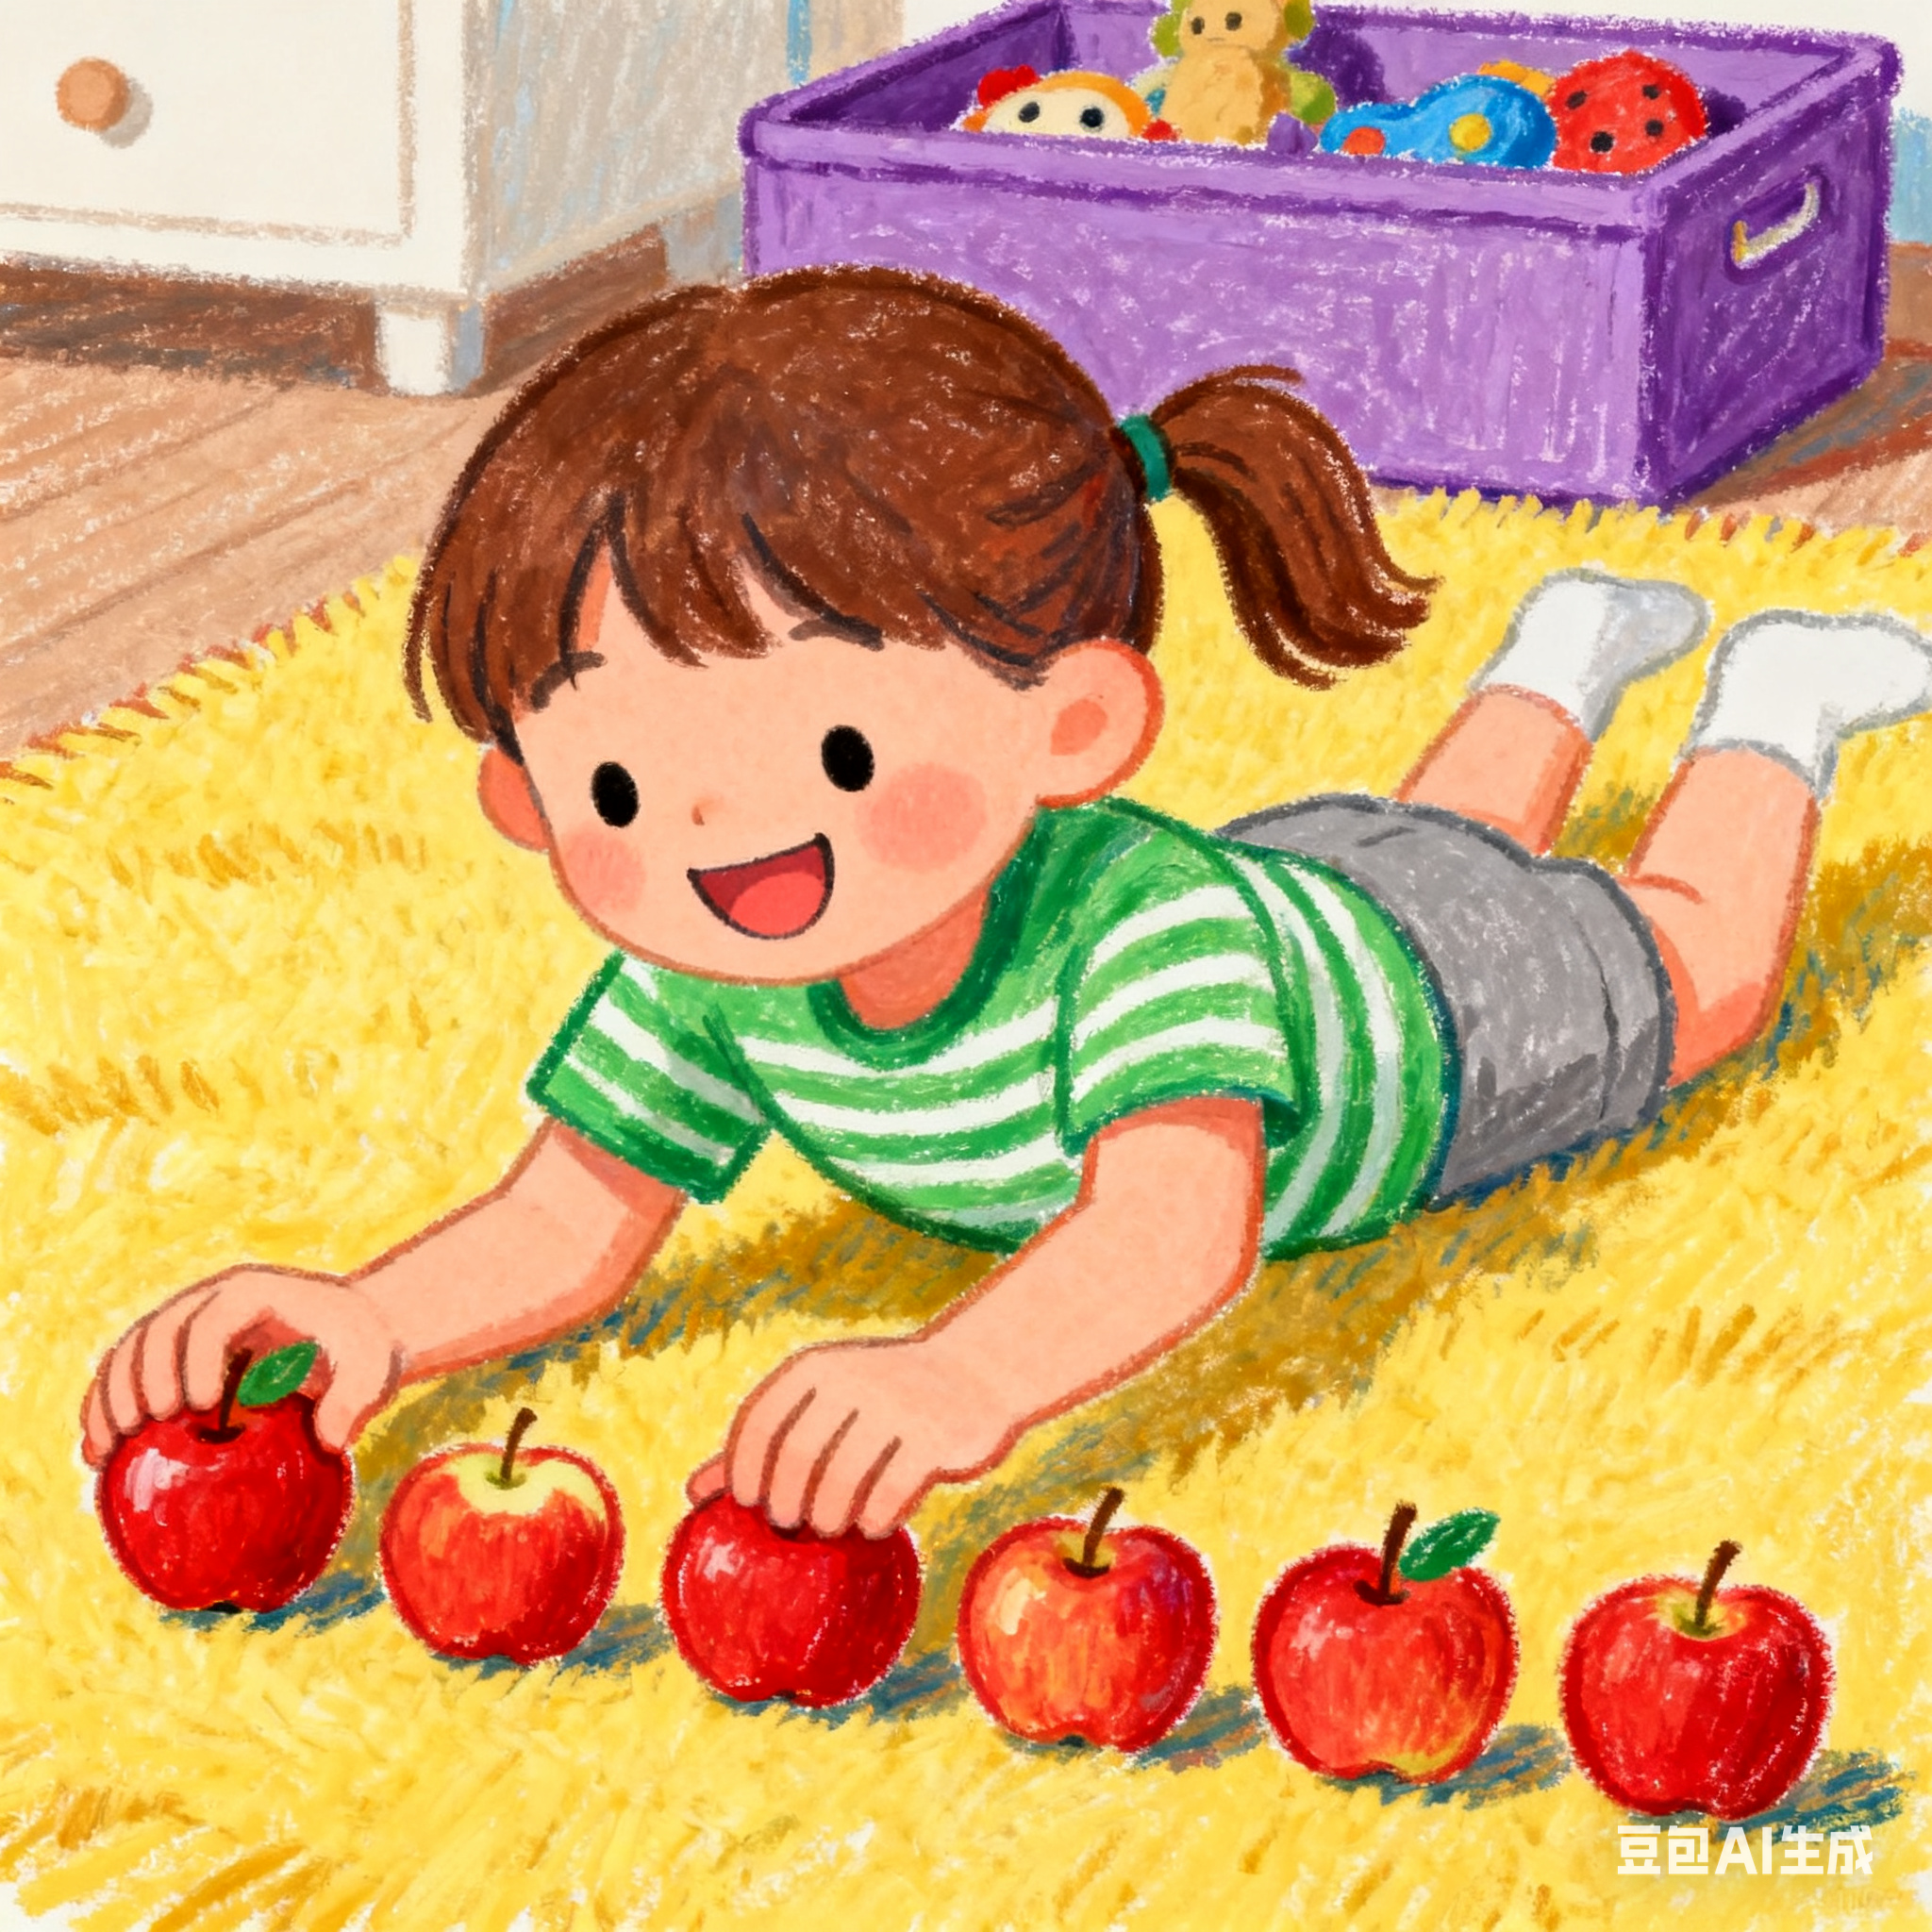
\includegraphics[width=0.8\textwidth]{countapple.png}
\paragraph{}如果是你,你可能会说:1, 2, 3, 4, \dots这样一直数,数出来的数就是自然数。
\paragraph{}我国高考遵循\textbf{国际标准 ISO 80000-2(the set of natural numbers, the set of positive integers and zero)}和\textbf{国家基础教育教材}的规范自然数包含0,那就是从0开始数,一直数出来数是自然数。
\paragraph{}说得没错,自然数就是你说的那些,而且只有那些,完全正确。
\section{再认识自然数}
\paragraph{}我现在化身杠精,想问问为什么从0开始数,数出来数是自然数,凭什么?老祖宗都说了:一生二,二生三,三生万物,从1数才是正解,才是自古以来。你只数到4,那5是不是自然数,9.9是不是自然数,很多是不是自然数,数不清是不是自然数......?总之,说从0数,数出来的数是自然数,我就是不服。
\subsection{从哪开始数}
\paragraph{}现在就0属不属于自然数,分为三个派别。第一个派别:传统派。认为0不属于自然数,这个派别应该是最古老的派别。你想,你数数会先数个0吗?会那么数的,C程序员无疑。打印字符串hello world!每个字符。
\begin{lstlisting}
	#include <stdio.h>
	int main() {
		char *str = "hello world!";
		
		for (int i = 0; str[i] != 0; i++) {
				printf("%c", str[i]);
		}
		return 0;
	}
\end{lstlisting}
\paragraph{}后来呢,像我这种懒人,偏听偏信的懒人多了,就发展出第二种派别:骑墙派。数数是从1开始数,那时候我是传统派。老师说高考定义是从0开始数,那时我就不是传统派。主打一个其乐融融,不惹事。
\paragraph{}那为什么把0加入到自然数,变成现在的正统了呢?那就要说到最后一个派别:集合论和逻辑学派。这个派别敬仰古希腊的荣光;就如同谈到西方政治,必然会有罗马帝国的痕迹。不论是希特勒第三帝国的建筑、艺术,还是美国政治人物的傲慢、自负,都似乎带着向罗马帝国致敬的味道,认为自己是伟大历史的书写者。古希腊的理性、思辨是人类的第一次觉醒,它塑造了现代文明:理性主义(不偏听偏信)、人文主义(生而平等)、公民意识(一切归劳动者所有,哪能容得寄生虫!)。看到上面说的是不是热血沸腾,会不会感觉古希腊的荣光还不够亮。
\paragraph{}\includegraphics[width=0.8\textwidth]{liberty_leading_people.png}
\paragraph{}一帮做数学的,也年轻过,也中二过,他们认为开创历史不是梦。他们从古希腊继承了有一部传世之作《几何原本》。我们作为普通人生活在距离这本书2300年后的今天,生活中99\%的数学问题,都可以从中找到解决方法。这本书让人惊叹的地方是:它只依赖5 条公理(适用于所有学科的基本真理,如 “等于同量的量彼此相等”)和 5条几何公设(如“过两点能作且只能作一直线”“直角都相等”),也就是只要承认5条公理5条几何公设,通过严格的逻辑推导,必然能够证明 465 个命题,它涵盖平面几何、立体几何、数论等领域。

% 公理部分
\begin{tcolorbox}[theorembox, title={5条公理}]
	\begin{enumerate}[label=\arabic*., leftmargin=*, noitemsep]
		\item 等于同量的量相等。
		\item 等量加等量,其和相等。
		\item 等量减等量,其差相等。
		\item 重合的量相等。
		\item 整体大于部分。
	\end{enumerate}
\end{tcolorbox}

\vspace{10pt} % 两个框之间的间距

% 公设部分
\begin{tcolorbox}[theorembox, title={5条公设}]
	\begin{enumerate}[label=\arabic*., leftmargin=*, noitemsep]
		\item 从任一点到任一点可以引一条直线。
		\item 有限的直线可以无限延长。
		\item 以任一点为中心,任意距离可以画圆。
		\item 所有直角都相等。
		\item 若一条直线与两条直线相交,且在同侧的两个内角之和小于两个直角,则这两条直线无限延长后,会在该侧相交。
	\end{enumerate}
\end{tcolorbox}
\paragraph{}于是集合论和逻辑学派的那帮人就思考,他们能不能也从几条基础的公理出发,根据逻辑推导最后重新建立数学大厦。
\paragraph{}初高中可能学了集合,可是会有种感觉:集合也就那么回事,好像什么事也没发生。对了,这种感觉对了。集合如果不和逻辑发生关系,它什么都不是。正是有了推导,才会有新的发现,美妙的启发。大部分的人的推导需要逻辑的约束,少部分人是不需要,比如女朋友、女朋友们、女朋友们的闺蜜们”。
\paragraph{}很多人说我也学过逻辑啊,辩证法不是逻辑吗?辩证法是我评价问题,指导行动的逻辑;所有的事物和变化发展规则都是对立统一、两个方面螺旋运动,内外力共同作用的结果。我要说的是:bi你bi的狗屁,但凡有人让你辩证的看待某个问题时,那他开始要不讲道理了。对(真)就是对(真),错(假)就是错(假),幼儿园老师、父母就是这样教的。bi人放火,打家劫舍就是错的,还辩证个屁。世界只有真和假,没有半真半假、即真又假。即真又假是岳不群、林平之。(这段话钟毅康表示不赞同、反对,但对于我个人观点给予尊重)
\paragraph{}学了逻辑后,有些人假话说得比真话多,学习让那些人变得狡猾。知道吗?说假话让你怎么说都是有对的地方;而说真话有一半的概率,会是错的。
\paragraph{}\underline{说假话,然后得出假的结论},别人会说:你说得好有道理。比如:
\begin{align}
	& 1 + 1 = 3 & \text{假条件} \label{c01:1}\\
	& (1 + 1)_3 + 1 = 3 + 1 & \text{\ref{c01:1}两边加1} \label{c01:2} \\
	& 3 + 1 = 4  & \text{\ref{c01:2}右边计算加法}
\end{align}
如果1+1=3,那么3+1=4,没错吧。
\paragraph{}\underline{说假话,然后得出对的结论},别人会说:你说得没错,赞。比如:
\begin{align}
	& 1 + 1 = 3  & \text{假条件} \label{c01:3}\\
	& \quad \ \ 0 = 1      & \text{\ref{c01:3}两边减2} \label{c01:4}\\
	& 1 + 1 = 2  & \text{\ref{c01:3}两边减\ref{c01:4}的两边}
\end{align}
如果1+1=3,那么1+1=2,没错吧。
\paragraph{}也就是,说假的前提,你怎么说都能给圆回去。古训说的:一句谎言,十句圆谎;十句谎言,一生难偿。古训欺负老实人嘛。
\paragraph{}说真话,必须得到真的结论,不然一下就穿帮了。比如你说1+1=2的话,1+1+1=4。别人会说:睁眼说瞎话嘛。
\paragraph{}既然这么容易被耍,后来人们就想了个办法,就是把结论当前提,看能不能圆回去(下图P$\Leftrightarrow$Q)。成功降低了被骗的概率。
\begin{table}[ht]
	\centering
	\caption{逻辑推导真值表}
	\label{tb:reduce}
	\begin{tabular}{cccccc}
		\toprule
		$P$ & $Q$ & $P \Rightarrow Q$ & $\neg$Q $\Rightarrow$ $\neg$P & $P \Leftrightarrow Q$ \\
		\midrule
		T & T & T & T & T \\
		T & F & F & F & F \\
		F & T & T & T & F \\
		F & F & T & T & T \\
		\bottomrule
	\end{tabular}
\end{table}
\paragraph{}$\iff$是个两头都有箭头的符号,箭头代表推导;$\Rightarrow$(向右的箭头)表示左边的情况如果满足,那么右边必然也满足;同理$\Leftarrow$(向左的箭头)表示右边情况满足,左边必然也满足。T表示真,F表示假,$\neg$表示反转。
\paragraph{}查看\eqref{tb:reduce},发现了一个规律,就是P$\Rightarrow$Q和$\neg$Q$\Rightarrow$$\neg$P,它们的真假值是一样的,一个命题和它的逆否命题真假一致。这个方法非常重要,当证明一个问题时,正面攻克不了,就攻克它的逆否命题。不过对于我这种“地瓜”智商,正面攻克不了,逆否也是白搭。我主要用这种方法写小作文,因为搞文学的人和小女生都喜欢这种不好好说的话。比如“我爱你”,变成命题形式:如果有个人是我,那么这个人爱你,现在改成逆反命题:如果一个人不爱你,那么,这个人不是我。经过逆否命题一改,字多了,诚意也多;这么绕,能把他们绕晕。逆反命题值得一练。
\begin{table}[ht]
	\centering
	\caption{非的真值表}
	\label{tb:neg}
	\begin{tabular}{cccccc}
		\toprule
		$P$ & $\neg$P \\
		\midrule
		T & F \\
		F & T \\
		\bottomrule
	\end{tabular}
\end{table}
\paragraph{}集合是把一类东西放一起,就像放学排入队,一群学生站一起;一堆苹果放一个货架上。放一起的东西各式各样,那取个名字吧,叫\underline{元素}。其实把元素叫东西也可以,但刚好集合的是一群人,叫东西就有些侮辱人了。干脆叫元素,反正你也没听说过,挑不出我毛病。
\paragraph{}看,多完美,我只是定义了一个框和东西,我们就可以开始数数了。等等,从哪里开始数呢,一开始集合里就有东西吗,有多少?数学家就想:从哪里开始数呢?就像《几何原本》它的需要5条公理5条公设,那数学需要的基础也是越少越好,难怪说数学家有洁癖。专业的人一般对自己的专业会有洁癖,表现得专业。比如我就看不惯函数4层以上的嵌套,goto乱来。洁癖和犟种的区别是,犟种不是蠢就是自卑。洁癖的数学家说:干脆从什么都没有开始,多干净。这个意见获得了数学家的共识。于是一条公理被提了出来:存在不含任何元素的集合。也就是别吵了,从0开始数。
\subsection{数学语言}
\paragraph{}这里插播一下。大部分人上大学后会发现,大学的数学书看不懂了。那其实是,近代数学公理化之后,同行之间开始用黑话交流。

{\itshape
“天王盖地虎,宝塔镇河妖”:这是《林海雪原》中最经典的黑话对答,是杨子荣假扮土匪时与座山雕手下的接头暗号。
“天王盖地虎” 意为 “你好大的胆子,敢来欺辱你祖宗?”
“宝塔镇河妖” 意为 “我若撒谎,让我被河水淹死,受宝塔镇压。”
“西北玄天一朵云,乌鸦落在凤凰群”:形容自己人来到了厉害的团伙中,下句接 “满桌都是英雄汉,谁是君来谁是臣?” 用于试探地位。

这是现代互联网里的黑话:我们要从顶层设计出发,聚焦用户痛点,通过差异化策略和精细化的颗粒度运营,击穿用户心智,打造产品的核心竞争力。在这个过程中,要注重各个环节的拉通和对齐,形成完整的业务闭环。同时,以数据为抓手,进行抽离透传和归因分析,为决策提供有力支持,不断赋能业务发展,最终实现业务的持续增长,在行业中构建起我们的生态优势。
}

看到互联网黑话,我就倒胃恶心;能不能好好说话!用模糊、新概念掩盖自己空洞,掩盖自己对具体问题毫无处理方法。一句话就是:无能。数学是由最聪明的一群人推动的,它的黑话不是无能,而且为了应对杠精,从源头把傻缺给排除。所以没有刻意训练数学的语言,当然是看不懂近代数学。好好学习这门语言吧,它会比英语更加通用,流传会更加悠远。更重要的是,学好后,你有资格和村口的大妈华山论剑,一决高下。

\begin{mdframed}[
	linewidth=1pt
	]

\quad \quad 我们说:元素、集合

老外说:element、set

数学说:我用小写字母a、b、x等表示元素,用大写字母A、B、C等或者用\{\}表示集合;而空集如此特殊,被定义为这个符号:$\emptyset$。
\end{mdframed}
\paragraph{}$\emptyset$是象形文字,用圆圈表示围起来的集合,用斜线划去表示什么都没有。例如一个包含a、b、c元素的集合A:\{a、b、c\}。
\begin{center}
	\begin{tcolorbox}[
		colback=white,
		colframe=blue!50!black,
		arc=3mm,
		boxrule=1pt,
		width=0.7\textwidth, % 框的宽度
		center, % 框内内容居中
		enlarge left by=0mm,
		enlarge right by=0mm,
		top=3mm,
		bottom=3mm,
		]
		空集公理:存在不含任何元素的集合。
		
		数学语言:$\exists$$\emptyset$$\forall$x(x $\notin$ $\emptyset$)
	\end{tcolorbox}
\end{center}
\paragraph{}上面的数学语言就是那批向古希腊致敬的数学家发明的,为了表达颠覆他们时代的意味,集合论里大部分成对关系的符号是倒影,或者是正常符号的翻转,空集公理的数学语言里有两个符号是正常符号翻转得来的。发现了吗:$\exists$、$\forall$。
\paragraph{}$\exists$左右旋转后是E,它源自拉丁语Existere的第一个字母。“Existere” 在拉丁语中由前缀 “ex-”(意为 “出、向外”)和词根 “sistere”(意为 “站立、存在”)组成,英语的exist(存在)就是这么来的。这个符号表的意思是:我就光明正大的站在这里。一般我们把他读作“存在”。存在就存在,有什么用呢?用处非常大,行走江湖抬杠必备。比如有人说:鸟都会飞。你说:存在一种鸟不会飞:鸵鸟。有人说:食物都会变馊。你说:存在一种食物不会变馊:蜂蜜。学会了吧,但凡别人说全部都怎么样,你只要举出$\exists$(存在)的一种反例,就能把他怼死。这就是$\exists$(存在)存在的意义。
\paragraph{}有认识$\forall$的朋友说:$\forall$是A的上下旋转,因为$\forall$的意思是“所有的”,那就是All的第一个字母。意思是对的,很可惜,来历不是这样的。它确实是所有的意思,但它是由拉丁语 “Omnis”(意为 “所有的、每一个”)的第一个字母得来的。我也无法理解$\forall$怎么就是O的旋转了,直到我看到o的手写体,为了连笔,o的左右俩边都有一个向下的线,上下旋转后变成向上的线,就变成了$\forall$。 $\forall$的目的是扩大打击面,就像《破坏之王》里的空手道大师兄“断水流”的经典台词:我不是针对你,我是说,在座的各位$\forall$都是勒色。又比如:你指出某些东西的不好,这时有人就说:\underline{任何}说**不好,$\forall$都是*黑。一般$\forall$可以用:“都”、“全部”、“任何一个、任意拿出一个”来表述,用“任何一个、任意拿出一个”表述最自然,最接近我们日常表达。
\paragraph{}上面的空集公理就还剩下最后一个符号了。$\notin$很明显那条斜线就是否定的意思,去掉斜线后是$\in$。$\in$源于拉丁语 “est”(某物是某集合的元素,即 “某物属于某集合”),这个单词和英语的“is”同一个意思。但我们不能简单的翻译成“是”,因为我们的“是”是等同的意思,而数学中,这个符号更准确的意思是“属于”、“是集合中的元素”。这个符号表示了元素和集合的关系。x$\in$A:x是A集合里的元素。x$\notin$A:x不是A集合里的元素。这里有个小细节,加上这个小细节,空集公理的数学语言我们就完全可以读懂了。这个细节是我们把可以改变的元素,用x、y、z这种小写字母表示,而用a、b、c这种小写字母表示不会改变的元素。
\paragraph{}重读空集公理:$\exists$$\emptyset$$\forall$x(x $\notin$$\emptyset$)。直译:存在空集和所有的元素,所有的元素都不属于空集。再译:存在空集和所有元素,从所有元素中取出任何元素,这个元素都不属于空集。说人话就是:存在空集,空集里不包含任何元素。
\paragraph{}好啦,废话一堆。目的就是说:从空集公理出发,我们的自然数从0开始数。空集里没元素,没有任何东西,我们就说空集表示0。
\subsection{我会数数了}
\paragraph{}有0了,那1是不是也要定义一个区别$\emptyset$的集合,叫1集合?为了遵循“如无必要,勿增实体”的原则,死犟死犟的数学家什么都没引入,他把空集再用了一遍来表示1。我想到的是这种\{$\emptyset$\}。漂亮!这种表示1,无懈可击。接着来2,\{$\emptyset$、$\emptyset$\}。
\paragraph{}嗯......这个2的集合表示好像碰到了点问题。什么问题呢?举个例子:把家庭成员里,会打乒乓球的人组成一个集合,这个集合是A:\{我、弟弟\};把家庭成员里,是程序员的人组成一个集合,这个集合是B:\{我\}。现在把家庭成员里,会打乒乓球的人和程序员组成一个集合C。这个集合C是\{我、弟弟\},还是\{我、弟弟、我\}呢?很明显,看上去它们是有区别的,但实质上它们描述的是同一个事物。也就是集合中相同的元素即使重复多次,对集合的整体没有影响。
\paragraph{}那2到底要如何从上面仅有的元素、集合、空集的概念推导出来呢?$\emptyset$和$\emptyset$是同一个,然而$\emptyset$和\{$\emptyset$\}不是同一个。那2就可以用\{$\emptyset$、\{$\emptyset$\}\}表示。
\paragraph{}到这,我似乎发现了获得下一个集合的规律。把当前集合元素的所有元素合并到下一个集合,再加上一个“当前集合”的元素(集合作为元素)。
\begin{itemize}[label=]
	\item 0:$\emptyset$ $\rightarrow$ 把$\emptyset$作为下一个集合的元素
	\item 1:\{$\emptyset$\} $\rightarrow$ \underline{\{$\emptyset$\}}
	\item 2:\{$\emptyset$、\underline{\{$\emptyset$\}}\} $\rightarrow$ \underline{\{$\emptyset$、\{$\emptyset$\}\}}
	\item 3:\{$\emptyset$、\{$\emptyset$\}、\underline{\{$\emptyset$、\{$\emptyset$\}\}}\} $\rightarrow$ \underline{\{$\emptyset$、\{$\emptyset$\}、\{$\emptyset$、\{$\emptyset$\}\}\}}
\end{itemize}
\paragraph{}漂亮,后面的4、5、6\dots 不是问题了,按照规则数下去都能得到。 
\subsection{先填一个坑}
\paragraph{}首先要填的第一个坑就是:明明可以用一次加一个$\emptyset$的方式来创造自然数,也就是集合里有1个空集,表示1,两个空集表示2的这种方式来表示自然数。为什么舍近求远,你不能用“我是我,独一无二的我”这个口号来灌输我错误的观念,说得好听,我是被卖家秀骗过的人,我要解释!很遗憾,没法给出解释,真没办法给出解释。
\paragraph{}数学家对没办法解释的事物,处理办法相当简单粗暴。没办法解释是吧,那就提出一个公理:
\begin{center}
	\begin{tcolorbox}[
		colback=white,
		colframe=blue!50!black,
		arc=3mm,
		boxrule=1pt,
		width=0.9\textwidth, % 框的宽度
		center, % 框内内容居中
		enlarge left by=0mm,
		enlarge right by=0mm,
		top=3mm,
		bottom=3mm,
		]
		外延公理:两个集合的元素相等,那么这两个集合相等。
		
		数学语言:$\forall X \forall Y (\forall x (x \in X \iff x \in Y) \iff X = Y)$
	\end{tcolorbox}
\end{center}
\paragraph{}说实话,我一看到外延公理,我的第一反应是什么鬼。我说的不是,我不能理解外延公理的内容,而是“外延”这个词。“外延”是什么?能不能取个一目了然的名字:元素公理。等我带着这个问题,查看了“外延(extension)”、“内涵(intension)”的意思才知道,这两个词是一对,而且它们是哲学词汇。集合论的创立者“康托”在大学学习的是数学和哲学,那就难怪这公理的名字怪哲学,不是凡人可以明白。简单的说:“内涵”是我们的描述;“外延”是根据描述,能得到的东西。就例如:小于4的自然数是内涵,外延是\{0、1、2、3\}。从内涵你就能得出外延,但从外延不一定能得到你要的内涵。例如从外延\{0、1、2、3\},有人认为是小于4的自然数,有人认为是前4个自然数。使用内涵表示集合,甚至引发悖论,罗素悖论是个很有名的内涵悖论的例子。从上面的解释可以看出,要获得准确的、直接的信息,应该提取的是外延。在集合里,也就是元素。

{\itshape
有一个很有名的内涵悖论:罗素悖论。
	\begin{itemize}[label=$\bullet$]
		\item 某理发师宣称:“我只给所有不给自己理发的人理发。”	
		\item 请问:这个理发师该不该给自己理发。
		\begin{itemize}[label=$\circ$]
			\item 若他给自己理发,则违反 “不给自己理发” 的原则;
			\item 若他不给自己理发,则根据原则应给自己理发。
		\end{itemize}
	\end{itemize}
}
\paragraph{}接着来看看数学语言,有了上面学习数学语言的基础,重读外延公理:任意的两个集合A和B,任何的一个元素,只要这个元素在A里,那么这个元素必然也在B里;只要这个元素在B里,那么这个元素必然也在A里。那么我们说集合A等于集合B。倒回来,任意的两个集合A、B,A等于B,那么A的所有元素在B里,B的所有元素在A里。
\paragraph{}如果认为\{$\emptyset$\}代表1,\{$\emptyset$、$\emptyset$\}代表2,利用外延公理可以推导出1=2的悖论。
\begin{proof}
	把\{$\emptyset$\}记作X,把\{$\emptyset$、$\emptyset$\}记作Y。
	\begin{itemize}[label=]
		\item  \{$\emptyset$\}的所有元素是$\emptyset$。满足$\emptyset$ $\in$ \{$\emptyset$、$\emptyset$\};即$\forall$x(x$\in$X $\Rightarrow$ x$\in$Y)。
		\item \{$\emptyset$、$\emptyset$\}的所有元素是$\emptyset$、$\emptyset$。第一个$\emptyset$满足$\emptyset$ $\in$ \{$\emptyset$\},第二个$\emptyset$满足$\emptyset$$\in$ \{$\emptyset$\};即$\forall$x(x$\in$X $\Leftarrow$ x$\in$Y)。
		\item 根据外延公理:$\forall X \forall Y (\forall x (x \in X \iff x \in Y) \iff X = Y$。
		\item 得证\{$\emptyset$\} = \{$\emptyset$、$\emptyset$\}
	\end{itemize}
\end{proof}
所以根据配对公理,用\{$\emptyset$、$\emptyset$\}表示2不是可取的方法。
\subsection{再填一个坑}
\paragraph{}回顾上面说的创造下一个集合的规律:是把当前集合元素的所有元素合并到下一个集合,再加上一个“当前集合”的元素(集合作为元素)。

\begin{itemize}[label=]
	\item 0:$\emptyset$ $\rightarrow$ 把$\emptyset$作为下一个集合的元素。
	\item 1:\{$\emptyset$\} $\rightarrow$ \underline{\{$\emptyset$\}}
	\item 2:\{$\emptyset$、\underline{\{$\emptyset$\}}\} $\rightarrow$ \underline{\{$\emptyset$、\{$\emptyset$\}\}}
	\item 3:\{$\emptyset$、\{$\emptyset$\}、\underline{\{$\emptyset$、\{$\emptyset$\}\}}\} $\rightarrow$ \underline{\{$\emptyset$、\{$\emptyset$\}、\{$\emptyset$、\{$\emptyset$\}\}\}}
\end{itemize}
\paragraph{}首先要解决的第一个问题:两个集合必然能组成一个集合。这是我们从空集出发创造新集合做的第一个动作,我们需要把它合法化。遇事不决,出公理:
\begin{center}
	\begin{tcolorbox}[
		colback=white,
		colframe=blue!50!black,
		arc=3mm,
		boxrule=1pt,
		width=0.9\textwidth, % 框的宽度
		center, % 框内内容居中
		enlarge left by=0mm,
		enlarge right by=0mm,
		top=3mm,
		bottom=3mm,
		]
		配对公理:任意的两个集合a、b能组成新的集合C=\{a、b\}。
		数学语言:$\forall$a $\forall$b $\exists$C $\forall$x(x $\in$ C $\iff$ (x = a $\lor$ x = b))
	\end{tcolorbox}
\end{center}
\paragraph{}读数学语言:这句数学语言出现了新的符号:$\lor$,它读作“或”、“或者”。它的来源是拉丁语“vel”(或)的首写字母v。记不住的话,就把$\lor$当成一个坑,或者这个或者那个都可以往里边丢。它的用法是只要$\lor$的左右两边有一个有效就认为“$\lor$左右两边”这个整体有效。比如别人问你:什么时候踢进世界杯?你可以回答:草坪太干或者草坪太湿或者草坪不干不湿,我都会输球。说得输球好像不是你的问题,是草坪的问题。草坪那么多或者的情况,只要满足一条,你就可以输球。用数学的语言把配对公理读出来就是:任意两个集合(两个形成配对,所以叫配对公理),存在第三个集合,第三个集合里的任何一个元素是前面两个集合之一。
\paragraph{}配对公理只是解决了两个集合能组成第三个集合,而且第三个集合里的元素是前两个集合。我们通常把这种“集合的元素是集合”的集合称为集合族。其实应该叫集合群,也就是一群集合组成的集合,但群在数学已经被伽罗瓦提前占位了,族群、族群,只剩下族了,所以我们把这类集合叫集合族。虽然两个集合组成第三个集合已经合法化,但我们通常更加关注的是把前两个集合的元素打散放到第三个集合,也就是合并两个集合的元素。
\begin{center}
	\begin{tcolorbox}[
		colback=white,
		colframe=blue!50!black,
		arc=3mm,
		boxrule=1pt,
		width=0.9\textwidth, % 框的宽度
		center, % 框内内容居中
		enlarge left by=0mm,
		enlarge right by=0mm,
		top=3mm,
		bottom=3mm,
		]
		并集公理:存在一个集合,它的元素是集合族里集合的元素。
		
		数学语言:$\forall$X $\exists$Y $\forall$u(u $\in$ Y $\iff$ $\exists$z(z $\in$ X $\land$ u $\in$ z))
	\end{tcolorbox}
\end{center}
\paragraph{}读数学语言:这里又出现了一个数学符号$\land$,它刚好和我们从配对公理学的$\lor$方向相反。$\lor$是或者的意思,相反的$\land$是而且的意思。比如很多男人说的“肤白貌美大长腿”,是或者的意思,只要有一个满足就是美女;很多女人说的“有车有房”才结婚,是而且的意思,必须有车而且有房,都达到了才满足条件。严以律己、宽以待人说的是对自己要用而且,对别人要用或者。现在这句古训慢慢被另一句话替代:我也是第一次做人,凭什么?先通读一遍$\forall$X $\exists$Y $\forall$u(u $\in$ Y $\iff$ $\exists$z(z $\in$ X $\land$ u $\in$ z)),从z $\in$ X $\land$ u $\in$ z可以看出来,X是一个集合族,因为X的元素是z,而z的元素是u,也就是z是一个集合,X的元素是集合z。有了这些信息,从头开始读:任何的集合族,都存在一个集合,这个集合的元素是集合族里集合的元素。
\begin{definision}
	集合的并运算 X $\cup$ Y 定义为:
	\[
	X \cup Y = \{ x \mid x \in X \lor x \in Y \}
	\]
\end{definision}
集合的并,就是把集合的所有元素提取出来,放入新的集合作为元素。现在可以让我们根据配对公理和并集公理,构造从0 $\rightarrow$ 1 $\rightarrow$ 2 $\rightarrow$ 3了。
\begin{itemize}[label=]
	\item 0:$\emptyset$
	\item 1:\{$\emptyset$\} $\rightarrow$ \underline{\{$\emptyset$\}}
	\item 2:\{$\emptyset$、\underline{\{$\emptyset$\}}\} $\rightarrow$ \underline{\{$\emptyset$、\{$\emptyset$\}\}}
	\item 3:\{$\emptyset$、\{$\emptyset$\}、\underline{\{$\emptyset$、\{$\emptyset$\}\}}\} $\rightarrow$ \underline{\{$\emptyset$、\{$\emptyset$\}、\{$\emptyset$、\{$\emptyset$\}\}\}}
\end{itemize}
\paragraph{}构造从0 $\rightarrow$ 1。有两个集合$\emptyset$、\{$\emptyset$\},根据并集公理,必然有一个集合,这个集合的元素是两个集合的元素。$\emptyset$没有元素,\{$\emptyset$\}的元素是$\emptyset$,所以构造的集合是\{$\emptyset$\}。
\paragraph{}构造从1 $\rightarrow$ 2。有两个集合\{$\emptyset$\}、\{\{$\emptyset$\}\},根据并集公理,必然有一个集合,这个集合的元素是两个集合的元素,\{$\emptyset$\}集合的元素是$\emptyset$,\{\{$\emptyset$\}\}集合的元素是\{$\emptyset$\},所以构造的集合是\{$\emptyset$、\{$\emptyset$\}\}。
\paragraph{}构造从2 $\rightarrow$ 3。有两个集合\{$\emptyset$、\{$\emptyset$\}\}、\{\{$\emptyset$、\{$\emptyset$\}\}\},根据并集公理,必然有一个集合,这个集合的元素是两个集合的元素,\{$\emptyset$、\{$\emptyset$\}\}的元素是$\emptyset$、\{$\emptyset$\},\{\{$\emptyset$、\{$\emptyset$\}\}\}的元素是\{$\emptyset$、\{$\emptyset$\}\},所以构造的集合是\{$\emptyset$、\{$\emptyset$\}、\{$\emptyset$、\{$\emptyset$\}\}\}
\paragraph{}根据上面的方法,就可以一直的构造自然数。从现在开始,我宣布“你可以合法的数数了”。
\subsection{填最后的坑}
\paragraph{}从上面构造自然数,我们采用了一种方法构造下一个自然数的方法:$x^{+} = x \cup \{x\}$。这种方法有个名称叫:\underline{归纳}。我们在生活中还经常碰到一个词:递归。递归就像内卷,当整个社会产生了内卷的氛围,这种氛围就像病毒一样蔓延到每个公司,公司再把这个病毒传递给每员工,员工又在不知不觉中传递到家庭,又从家庭传递给每一个人。递归是一种简单的方法,但它能触及到任何的角落。作为程序员可以不知道归纳,但万万不能不知道递归。程序的函数是指把一个过程组合成一个整体可以操作的对象。递归是在这个函数过程中,再次执行了这个函数。例如你要获取计算机所有的文件名称,下面的几行递归伪代码实现了这个目的。
{\itshape
	\begin{itemize}[label=]
		\item 遍历目录(需要遍历的目录路径) \{
		\begin{itemize}[label=]
			\item 打开需要遍历的目录路径
			\item 查看当前层级的文件和目录
			\item 如果是文件,那么收集这个文件名称
			\item 如果是目录,那么再次执行\large{遍历目录(这个目录路径)}
		\end{itemize}
		\item \large{遍历目录(我的电脑)}
	\end{itemize}
}
\paragraph{}\underline{递归采用的是从大往小递进;归纳正好相反,它是从小往大延伸。}仔细观察,生活中处处有递归和归纳,只要是一种能渗透进每个角落的传播方式,那它不是递归就是归纳,或者是两者震荡放大的结果。扶不扶摔倒的老人是归纳,买不买房是递归,内卷是从几家IT公司开始(You are shame)归纳到IT行业竞争氛围,然后通过氛围递归到整个社会。
\paragraph{}说了这么多,现在思考一个问题:归纳是一个过程,这个过程在自然数中是不会停止的,那需要怎么看待自然数。简单的说:把自然数看出一个过程,还是一个整体。也就是自然数是不是一个集合。小白会疑惑,这重要吗?当然,这关系到1 $\div$ 3 = 0.33$\dot{3}$ 里的0.33$\dot{3}$,你认为它是一个 真实存在的确切的数,还是一个过程。为了解决这个问题,再次提出了一个公理:
\begin{center}
	\begin{tcolorbox}[
		colback=white,
		colframe=blue!50!black,
		arc=3mm,
		boxrule=1pt,
		width=0.9\textwidth, % 框的宽度
		center, % 框内内容居中
		enlarge left by=0mm,
		enlarge right by=0mm,
		top=3mm,
		bottom=3mm,
		]
		无穷公理:存在由归纳产生的集合。
		
		数学语言:$\exists$S [$\emptyset$ $\in$ S $\land$ ($\forall$x $\in$ S)[x $\cup$ \{x\} $\in$    S]]
	\end{tcolorbox}
\end{center}
\begin{definision}
	$x^+ = x \cup \{x\}$,把$x^+$读作x的后继。以数字作为符号,定义后继:
	\[
		0^+ = 1 \quad 1^+ = 2 \quad 2^+ = 3 \quad \cdots
	\]
\end{definision}
\paragraph{}用数学语言读无穷公理:存在一个集合,空集是这个集合的元素,而且这个集合的元素的后继也是这个集合的元素。也就是从这个无穷公理开始,数学归纳法才真正合法。思考数学归纳法的步骤:命题的首项满足,如果命题的第n项满足的条件下,命题的第n项的后继也满足,那么我们说命题对全部($\forall$)自然数项满足。
\paragraph{}既然自然数是一个集合,而且这么重要的集合出去闯江湖。碰上鼠辈放肆,大吼一声:江湖道义岂容尔等践踏,藏头露尾非英雄,本人行不更名,坐不改姓,人称$\mathbb{N}$,Natural numbers的$\mathbb{N}$。一声枪响,$\mathbb{N}$卒,弹幕:“$\mathbb{N}$死于话多,下次别废话了!”
\section{有趣的自然数}
\paragraph{}我感觉这个章节,会很困惑,因为我们现在只有归纳一个工具,而且第一次讨论无穷。无穷它的一些性质颠覆了我们的很多固有想法,这个章节我们一块思考无穷情况下的问题。
\paragraph{}首先我们先做一个约定,我们接下来讨论的都是函数问题。当别人和你说:我们做个约定吧。这时请别光想着约定的美,还附带要放弃一部分自由呢。这里约定讨论函数问题,不仅仅是放弃我的自由,更重要的是我的智商只能勉强思考函数的问题。所以有些时候,放弃部分自由,其实是在保护自己。\dotuline{函数}问题之所以说简单,是因为它要求根据特定的输入,经过运算输出的\dotuline{结果只有一个},它非常符合认知。对于结果、目的、输出你不能既要又要。有一个结果就够了,只有围城内的才知道“一夫一妻”其实是在保护男性。既要又要的结果就是,没办法预测结果。函数的一个要求就是,结论,或者说输出唯一。这个唯一不是任何输入对应的输出的确切结果唯一,说的是在确定输入的情况下结果唯一。比如身份证,一个身份证号对应唯一的一个人,其他人的身份证号不对应这个人,指向其他的唯一的人。函数简单的说就像进动车站刷身份证,输入身份证信息和你的人脸,经人证合一的校验,输出唯一的结论:是你或者不是你,来决定让不让你进站。根据以上的分析,函数包含三个方面:输入非、运算、输出。而且特别要求,根据指定的输入,对应的输出是唯一的。
\begin{definision}
	函数是输入集合对应输出集合的一种关系,输入集合的一个元素,唯一地输出集合的一个元素。下列的符号定义F()表示函数运算,x表示输入,y表示输出。
	
	F(x, y):$\forall$x $\forall$y$_{1}$ $\forall$y$_{2}$[(f(x, y$_{1}$) $\in$ F $\land$ f(x, y$_{2}$) $\in$ F) $\Rightarrow$ y$_{1}$ = y$_{2}$]
\end{definision}
有了函数,我们就可以定义运算了。首先我们想到的是什么?当然是加、减、乘函数。
有了函数还不够,因为我们关注的是自然数的函数。我们现在只有一个自然数集合,一个集合是无法满足函数的条件,需要两个集合输入集合和输出集合。那么现在我们需要从自然数分离出一个集合。由前面给的所有知识,都无法分离出一个集合,所以提出新的公理。
\begin{center}
	\begin{tcolorbox}[
		colback=white,
		colframe=blue!50!black,
		arc=3mm,
		boxrule=1pt,
		width=0.9\textwidth, % 框的宽度
		center, % 框内内容居中
		enlarge left by=0mm,
		enlarge right by=0mm,
		top=3mm,
		bottom=3mm,
		]
		分离公理:可以从任何集合中提取满足制定性质的元素,组成新的集合。
		
		数学语言:$\forall$A $\exists$B $\forall$x(x $\in$ B $\iff$ x $\in$ A $\land$ P(x))
	\end{tcolorbox}
\end{center}
\paragraph{}有了分离公理,我们可以提取自然数的数构成输入集合和输出集合。然后只剩下确保输出的唯一性,也就是归纳的输出要唯一。回顾归纳方法:$x^{+}=x\cup\{x\}$,做个假设,如果有一个集合它的元素是它自己,那么根据归纳方法和外延公理,归纳方法就会终结。
\paragraph{}因为我们不希望集合后继还是集合自己,所以我们需要确保:集合的元素不能是集合自己。
\begin{equation}
\textit{集合的元素不能是这个集合自己,即A $\neq$ \{A\}。} \notag
\end{equation}
\begin{Proof}
	用反证法证明:如果集合的元素还是集合自己,那么集合的后继还是自己。\\
	集合的元素还是集合自己:
	\begin{align}
		A&=\{A\} &&\quad \label{eq:selfcontained}
	\end{align}
	后继的定义:
	\begin{align}
		A^{+}&=A\cup\{A\} &&\quad \label{eq:successor}
	\end{align}
	把 \eqref{eq:selfcontained} 代入 \eqref{eq:successor}得到:$A^{+} = A \cup A$,根据集合的并运算和外延公理得到,得到$A^{+}=A$。
\end{Proof}
为了避免这个情况出现,再、再、再、再次提出一个公理。呜呜......数学越来越不美了,一碰到问题,就出一个公理,简直就是bug一般的存在。还能比黑人和原住民后代,性别认知障碍又有异装癖,素食又环保主义者buff叠满更无敌吗。
\begin{center}
	\begin{tcolorbox}[
		colback=white,
		colframe=blue!50!black,
		arc=3mm,
		boxrule=1pt,
		width=0.9\textwidth, % 框的宽度
		center, % 框内内容居中
		enlarge left by=0mm,
		enlarge right by=0mm,
		top=3mm,
		bottom=3mm,
		]
		正则公理:任意非空集合含有一个与自身不相交的元素。
		
		数学语言:$\forall$X(X $\neq$ $\emptyset$ $\Rightarrow$ $\exists$x(x $\in$ X $\land$ X $\cap$ x = $\emptyset$))
	\end{tcolorbox}
\end{center}
前面刚学了集合的并$\cup$,这里的$\cap$刚好是$\cup$的翻转,这两个符号是一对,$\cap$叫集合的交,$\cup$是把集合所有元素都提取出来组成新的集合;$\cap$是把两个集合\underline{相同}的元素提取出来组成新的集合。
\paragraph{}所以根据归纳方法和外延公理,集合符合正则公理的前提下,归纳不会终结,而且归纳产生的元素,是这个归纳集中独一无二的元素。对应自然数而言,自然数集合中的自然数个数是无穷的,每个自然数在自然数集合中独一无二。
\begin{definision}
	集合的交运算 X $\cap$ Y 定义为:
	\[
	X \cap Y = \{ x \mid x \in X \land x \in Y \}
	\]
\end{definision}
正则公理英文是Axiom of Regularity/Foundation,翻译英文叫规范公理或者基础公理。这里的规范和基础,说的是集合的规范和基础。
\paragraph{}根据正则公理$A \neq \{A\}$,那么$A^{+} \neq A \cup \{A\}$。对应到自然数:$x \neq x^{+}$,也就是自然数集合中的数与这个数的后继不相等。
\subsection{我会加法、乘法了}
\label{subsec:addmul} 
当我推理到有自然数的概念后。我认为可以这样解释加法:a+b是在自然数a的基础上执行b次的后继。是的,加法确实是以这种方式定义的。
\begin{definision}
	自然数的加法表示符合下列规则的函数$f_{+}$或者$f_{add}$,其中$x \in \mathbb{N} \land y \in \mathbb{N}$:
	\begin{empheq}[left=\empheqlbrace]{align}
		& x + 0 = x \tag{df.add.1}\label{df:add1} \\
		& x + y^{+} = (x + y)^{+} \tag{df.add.2}\label{df:add2}
	\end{empheq}
\end{definision}
这个定义表述得非常自然。一个任意数x加上另一个数,\eqref{df:add1}是任意数x加上另一个数的起点,然后反复\eqref{df:add2}的后继运算。例如我要算x+2。
\begin{align}
	x + 0 &= x & \quad \text{根据\eqref{df:add1}} \label{add:0}\\
	x + 1 &= (x + 0)^{+} = x^{+} & \quad \text{根据\eqref{df:add2}\eqref{add:0}} \label{add:1}\\
	x + 2 &= (x + 1)^{+} = ((x + 0)^{+})^{+} = (x^{+})^{+} & \quad \text{根据\eqref{df:add2}\eqref{add:1}}
\end{align}
上面的推导中,依赖数字作为符号的后继定义$0^{+}=1$、$1^{+}=2$。
\paragraph{}这个加法定义困扰了我很久,因为它有太多的问题值得思考:首先加法后的结果,能保证还是自然数吗?毕竟减法就产生了负数,除法产生了有理数,加法是如何保证运算后的结果在自然数范围内呢?其次加法符合函数的性质吗?也就是加后的结果唯一吗?
\paragraph{}到现在,我们的自然数还用着集合的、归纳的“表示”,“表示”是没用的,多少心爱的人都是被表示给耽误了。偷偷地看对方,她会认为我就是那么好看,别人也这样看她;酸溜溜的说:他是不是喜欢你。她会认为你打探她的隐私。直到你说,三十岁你还没结婚,我们凑合过吧。她暴怒,你在诅咒老娘嫁不出去是不是。表示不一定有用,也许别人认为你在养鱼。所以到了确定关系的时候了,大胆表白,不做舔狗。舔狗舔狗,添到最后一无所有。该给自然数下个定义了。
\paragraph{}这个定义是皮亚诺给的,也叫作皮亚诺公理,是公认的自然数的公理,满足下面皮亚诺公理的集合叫自然数集合$\mathbb{N}$,集合里的元素叫自然数。为了强调$x^{+}$的后继是一个数,后续会用S(x)表示$x^{+}$。另外新学一个逻辑符号$\exists$!,它的意思是“有且唯一”,中国有且唯一,大陆属于中国,台湾属于中国:$\exists$!中国(大陆$\in$中国 $\land$ 台湾$\in$中国)。有了$\exists$!这个符号,那么我们可以给出函数定义的简化版本:$\forall$x$\exists$!y(f(x,y) $\in$ F)。
\begin{enumerate}[label=\textbf{P\arabic*.}] 
	\item \textbf{0是自然数}($0\in\mathbb{N}$)。
	\item \textbf{每个自然数x,有唯一的S(x),S(x)也是自然数}($\exists!S(x)(x\in\mathbb{N} \land S(x)\in\mathbb{N})$)。
	\item \textbf{0 不是任何自然数的后继}($\forall x(x\in \mathbb{N} \land S(x) \neq 0)$)。
	\item \textbf{不同的自然数有不同的后继}($\forall x \forall y ((x \in \mathbb{N} \land y \in \mathbb{N} \land x \neq y) \Rightarrow S(x) \neq S(y))$)。
	\item \textbf{数学归纳法}:如果某个性质P满足:
	\begin{enumerate}
		\item P(0)成立,
		\item P(n) $\Rightarrow$ P(S(n)),\\
		则P对所有自然数成立。
	\end{enumerate}
\end{enumerate}
\paragraph{}皮亚诺公理可以由前面介绍的公理系统严格推导出来,例如P1和P3的简单推导:
\paragraph{}P1:由无穷公理定义$\mathbb{N}$,0=$\emptyset$,0是$\mathbb{N}$的一个元素。
\paragraph{}P3:如果0是某个自然数x的后继,那么0=x$\cup$\{x\}。0=$\emptyset$,根据配对公理、并集公理和外延公理只有x=$\emptyset$和\{x\}=$\emptyset$,但是x=$\emptyset$和\{x\}=$\emptyset$是矛盾的。
\paragraph{}明确了自然数的定义后,我们现在可以考虑第一个问题:自然数加法的结果能保证还是自然数吗?
\begin{equation}
	\textit{自然数加法的结果还是自然数} \label{nor:addstnor}
\end{equation}
\begin{Proof}
	根据加法规则($x \in \mathbb{N} \land y \in \mathbb{N}$):
\begin{empheq}[left=\empheqlbrace]{align}
	& x + 0 = x \tag{df.add.1}\label{df:add1} \\
	& x + y^{+} = (x + y)^{+} \tag{df.add.2}\label{df:add2}
\end{empheq}
\paragraph{}从\eqref{df:add1}可以看出来,这个规则已经帮我们解决了n=0的情况。
\paragraph{}当n=0时
\begin{align}
	x + n &= x + 0 & \quad \text{当n = 0} \label{add:n0}\\
	x + 0 &= x     & \quad \text{根据\eqref{add:n0}\eqref{df:add1}} \label{add:x0}\\
	(x + 0) &\in \mathbb{N} & \quad \text{根据$x \in \mathbb{N}$和\eqref{add:x0}} \label{add:y3}
\end{align}
\paragraph{}当n $\neq$ 0时,\itshape{归纳假设}:
\begin{equation}
	(x + n) \in \mathbb{N} \label{add:y0}  
\end{equation}
\paragraph{}证明($x+S(n)) \in \mathbb{N}$:
\begin{align}
	x + S(n) &= S(x + n) & \quad \text{根据\eqref{df:add2}}  \label{add:y1}\\
	S(x+n) &\in \mathbb{N} & \quad \text{根据\eqref{add:y0}和皮亚诺公理P2}  \label{add:y2}\\
	(x + S(n)) &\in \mathbb{N} & \quad \text{根据\eqref{add:y2} \eqref{add:y1}}  \label{add:y4}
\end{align}
\paragraph{}\eqref{add:y3}结论说明P(0)成立,\eqref{add:y0}和\eqref{add:y4}说明P(n) $\Rightarrow$ P(S(n))成立,由皮亚诺P5得出自然数x加上任意的自然数n,加出来的结果依然是自然数。
\end{Proof}
接着第二个问题:加法算出来的结果唯一吗?因为这直接关系到,加法是不是一个函数问题。
\begin{equation}
	\textit{自然数加法的结果唯一} \label{nor:addres1}
\end{equation}
\begin{Proof}
当n=0时
\begin{align}
	x + n &= x + 0 & \quad \text{当n = 0} \label{add:y15} \\
	x + 0 &= x     & \quad \text{根据\eqref{add:y15}\eqref{df:add1}} \label{add:y16}
\end{align}
\paragraph{}当n $\neq$ 0时,\itshape{归纳假设}:
\begin{equation}
	(x + n) \text{结果唯一} \label{add:y17}
\end{equation}
\paragraph{}证明(x + S(n))的结果唯一。
\begin{align}
	x + S(n) &= S(x + n) & \quad \text{根据\eqref{df:add2}} \label{add:y18} \\
	S(x + n) & \text{结果唯一} & \quad \text{根据\eqref{add:y17}和皮亚诺公理P2} \label{add:y19} \\
	(x + S(n)) & \text{结果唯一} & \quad \text{根据\eqref{add:y18}\eqref{add:y19}} \label{add:y20}
\end{align}
\paragraph{}\eqref{add:y16}结论说明P(0)成立,\eqref{add:y17}和\eqref{add:y20}说明P(n) $\Rightarrow$ P(S(n))成立,由皮亚诺P5得出自然数x加上任意的自然数n,加出来的结果是唯一的。
\end{Proof}
\paragraph{}第三个问题:是否存在一个除0外的自然数x,自然数n加上x后还是n?
\begin{equation}
	\textit{任意自然数n加上有且仅有0,还是n} \label{add:eq00}
\end{equation}
\begin{Proof}
	\begin{align}
		& \text{重述问题:n + x = n 是否为真} & \text{$x \in \mathbb{N}, n \in \mathbb{N}, (x \neq 0)$} \label{eq:nxn} \\
		& \text{$S(n + x) = S(n)$} & \text{根据\eqref{eq:nxn}和皮亚诺P2} \label{eq:nxn1} \\
		& \text{$n + S(x)$ = n + 1} & \text{根据\eqref{df:add2}\eqref{add:1}} \label{eq:nxn2} \\
		& \text{$S(0) = 1$} &\text{根据自然数定义}\label{eq:nxn3} \\
		& \text{$n + S(x)$ = n + S(0)} & \text{根据\eqref{eq:nxn2}\eqref{eq:nxn3}} \label{eq:nxn4} \\
		& \text{x = 0} & \text{根据\eqref{eq:nxn4}} \label{eq:nxn5} \\
		& \text{x = 0 \eqref{eq:nxn5}和x $\neq$ 0\eqref{eq:nxn}相矛盾} \label{eq:nxn6}
		\end{align}
根据证明得到:
	\begin{align}
			& \text{$n + x \neq n$} & \text{$x \in \mathbb{N}, n \in \mathbb{N}, (x \neq 0)$} \label{eq:nxn7}
	\end{align}		
\end{Proof}
\paragraph{}第四个问题:
\[
\begin{cases}
	a = b \\
	c = d
\end{cases}
\textit{是否可以$\implies$} a + c = b + d  \quad \text{($a, b, c, d \in \mathbb{N}$)}
\]
\begin{Proof}
证明a = b 则a + c = b + c。
\paragraph{}当c=0时
\begin{align}
	& \text{a + 0 = b + 0} & \text{根据\eqref{df:add1}}
\end{align}
\paragraph{}当c$\neq$0时,归纳假设:
\begin{equation}
	a = b \Rightarrow a + c = b + c \label{co:add1}
\end{equation}
\paragraph{}证明 a + S(c) = b + S(c)
\begin{align}
    & \text{a + S(c) = S(a + c)} & \text{根据\eqref{df:add2}} \label{co:add2} \\
    & \text{b + S(c) = S(b + c)} & \text{根据\eqref{df:add2}} \label{co:add3} \\
    & \text{S(a + c) = S(b + c)} & \text{根据\eqref{co:add1}和皮亚诺公理P4} \label{co:add4} \\
    & \text{a + S(c) = b + S(c)} & \text{根据\eqref{co:add2}\eqref{co:add3}\eqref{co:add4}}
\end{align}
证得
\begin{align}
\begin{cases}
	a = b \\
	c = d
\end{cases}
\text{$\implies$} a + c = b + d  \quad \text{($a, b, c, d \in \mathbb{N}$)} \label{co:add5}
\end{align}
\end{Proof}
\paragraph{}学会了加法,现在我们可以参加小学一年级期末考试啦,祝200个月的小朋友考试顺利。考试及格,欢迎加入乘法的学习。
\begin{definision}
	自然数的乘法表示符合下列规则的函数$f_{\times}$或者$f_{mul}$,其中$x \in \mathbb{N} \land y \in \mathbb{N}$:
	\begin{empheq}[left=\empheqlbrace]{align}
		& x \times 0 = 0 \tag{df.mul.1}\label{dmul:1} \\
		& x \times S(y) = x \times y + x \tag{df.mul.2}\label{dfmul:2}
	\end{empheq}
\end{definision}
\paragraph{}乘法也具有加法的函数性质,证明方法是一样的,我就不证明了。总结:自然数加法和乘法是自然数集合通过加法和乘法规则运算,映射到自然数集合的函数。直接给出以下结论:
\begin{equation}
	\textit{自然数乘法的结果还是自然数} \label{nor:mulnor}
\end{equation}
\begin{equation}
	\textit{自然数乘法的结果唯一} \label{nor:mulres1}
\end{equation}
\paragraph{}可以通过加法和乘法定义,以及数学归纳法证明以下运算规律:
\begin{align}
	x + y &= y + x & \quad \text{自然数加法交换律} \label{add:ex}\\
	(x + y) + z &= x + (y + z) & \quad \text{自然数加法结合律}  \label{add:asso}\\
	x \times y &= y \times x & \quad \text{自然数乘法交换律} \\
	(x \times y) \times z &= x \times (y \times z) & \quad \text{自然数乘法结合律} \\
	(x + y) \times z &= x \times z + y \times z \\
	 z \times (x + y) &= z \times x + z \times y  & \quad \text{自然数分配律}  \label{addmul:dis}
\end{align}
\begin{convension}
	当使用单个字母表示数时,它们的乘法可以简写为:$\cdot$或者直接省略。
	\begin{align*}
		\text{例如:} a \times b = a \cdot b = ab
	\end{align*}
\end{convension}
\subsection{一样,多了,少了?}
\paragraph{}在1998年《新华字典》修订本中有这样一个例句:“张华考上了北京大学;李萍进了中等技术学校;我在百货公司当售货员:我们都有光明的前途。”当年12岁的我,读了这句话,明白了什么是相等。首先,我的前途是光明的,光明的前途是我的。其次,我把售货员的前途给张华,张华欣然接受;张华把上北京大学的前途给我,我可以接受。再次,我把售货员的前途给张华,张华把上北京大学的前途给李萍,李萍把进中等技术学校的前途给我,我们都很开心。把它们总结为数学语言就是:
\begin{definision}
	集合X上的二元关系R,具有以下性质的关系称为\underline{等价关系}:
	\begin{align}
		& \text{所有的$x \in X$都有xRx。} \tag{自反性} \label{df:eqreflerive} \\
		& \text{所有的$x, y \in X$都有$xRy \Rightarrow yRx$。} \tag{对称性} \label{df:eqsymmetric} \\
		& \text{所有的$x, y, z \in X$都有$(xRy \land yRz) \Rightarrow xRz$。} \tag{传递性} \label{df:eqtransitive}
	\end{align}
\end{definision}
等价关系虽然简单,但是它却可以帮助我们认识新的运算。例如这个集合\{(0, 4), (1, 3), (2, 2), (3, 1), (4, 0)\},它蕴含集合\{0, 1, 2, 3, 4\}里加法和是4的等价关系:(a, b)R(c, d) $\leftrightarrow$ a + b = c + d = 4。也就是通过等价关系,我们可以推导出部分自然数的一种加法运算。后面的章节,我们利用等价关系,结合运算推导出新的数。
\begin{definision}
	x的等价类:
	\begin{align*}
		\text{所有与x满足关系R的元素组成的集合,记作$[x]_{R}$或简写为$[x]$。} \label{df:equivalenceclass}
	\end{align*}
\end{definision}
上面的$[(0, 4)]$ = \{(0, 4), (1, 3), (2, 2), (3, 1), (4, 0)\}是集合\{0, 1, 2, 3, 4\}里加法和是4的等价类。偶数也可以是一个等价类:$[0]$=\{0, 2, 4……\}。
\paragraph{}只要是具有等价关系,那么它们是可以相互替换的。例如在计算加法时,会把2+2替换为0+4,或者是化简后的4;除了算数运算时的替换,在证明时也会有替换,例如证明(x + S(n)) $\in$ $\mathbb{N}$\eqref{add:y4},把x + S(n) = S(x + n)\eqref{add:y1}等价的算式代入到S(x + n) $\in$ $\mathbb{N}$\eqref{add:y2};在逻辑推理时也会采用等价的方法,例如根据逻辑推理真值表\eqref{tb:reduce},结合非得真值表\eqref{tb:neg},那么会有(P $\Rightarrow$ Q)和($\neg$Q $\Rightarrow$ $\neg$P)真假值等价,这种逻辑等价给我们提供了更多,灵活多变的推导方式。
\paragraph{}除了等价的二元关系,还有一种二元关系和日常息息相关,那就是搞排名,比大小。假设有一家科技公司,它的营销费用占营收10\%左右,假设另一家取消传统营销部门的公司,它的营销费用占营收0.16\%。你认为在现实中,取消传统营销的公司,在营收更高的情况下,谁还有更多的钱投入研发、产品质量?如果两家科技公司宣传时,一家除了宣传科技价值,还强调附带特别的情绪价值,另一家仅仅推广科技价值,请问哪家公司的科技排名更靠前?真像成绩排名不好的我,成绩不够文具来凑,“差生文具多”说的是我。
\paragraph{}上面这种关系是偏序关系,它最显著的特点就是舍我其谁,我最最厉害,另一个我都不能和我比。
\begin{definision}
	集合X上的二元关系R,具有以下性质的关系称为\underline{严格偏序关系}:
	\begin{align}
		& \text{所有的$x \in X$都有x\cancel{R}x。} \tag{反自反性} \\
		& \text{所有的$x, y, z \in X$都有$(xRy \land yRz) \Rightarrow xRz$。} \tag{传递性}
	\end{align}
	\cancel{R}的意思是不存在关系。
\end{definision}
\paragraph{}小于号$<$和大于号$>$是我们常用的严格偏序符号,用于比大小,长短,轻重,排名。自然数的大小刚好可以利用刚学的加法来定义。
\begin{definision}
	任意自然数a、b, 当且仅当($\iff$)以下条件,那么a $<$ b 和 b $>$ a:
	\begin{equation}
		a + x = b  \quad \quad \text{$\exists x(x \in \mathbb{N} \land x \neq 0)$} \label{df:compare} \tag{df.n.order}
	\end{equation}
\end{definision}
\paragraph{}定义了大于、小于你就正式告别快乐的童年了。这时你会发现,父母的眼里永远有一类小朋友。他成绩大于你,乖巧懂事大于你,惹是生非小于你,他是你无法逾越的鸿沟,父母、老师眼中的榜眼,他是舞台上的明星、红旗下的花朵。他有个响亮的名字:领居家的小孩。其实不用担心,因为你也可能是其他父母眼中的那个领居家的小孩。

\paragraph{}\textit{对任意m,n $\in \mathbb{N}$,以下三种情况有且只有一个成立:}
	\begin{equation}
		m < n \quad \quad m = n \quad \quad m > n \label{nor:sort3}
	\end{equation}
\begin{Proof}
	证明只会有一种情况成立:
	\begin{itemize}[label=$\circ$]
	\item 当m $<$ n时:
		\begin{align}
			& m + x = n \quad \text{$\exists x(x \in \mathbb{N} \land x \neq 0)$} \quad & \text{根据\eqref{df:compare}} \label{pf:t1}\\
			& m \neq n & \text{根据\eqref{pf:t1}\eqref{eq:nxn7}} \label{pf:t2} \\
			& \text{假设 m $>$ n,则n + y = m} & \text{根据\eqref{df:compare}} \label{pf:t3} \\
			& n + y + x = n & \text{根据\eqref{pf:t3}\eqref{pf:t1}} \label{pf:t4} \\
			& \text{n + y + x $\neq$ n} & \text{根据\eqref{eq:nxn7}} \label{pf:t5} \\
			& \text{m $\cancel{>}$ n} & \text{根据\eqref{pf:t4}和\eqref{pf:t5}矛盾}
		\end{align}
	\item 当m = n时:
	\begin{align}
		& \text{$n + x \neq m$} & \text{根据m=n和\eqref{eq:nxn7}} \label{pf:t6} \\
		& \text{m $\cancel{<}$ n} & \text{根据\eqref{pf:t6}\eqref{df:compare}} \\
		& \text{m $\cancel{>}$ n} & \text{根据\eqref{pf:t6}\eqref{df:compare}}
	\end{align}
	\item 当m $>$ n时:
		\begin{align}
		& n + x = m \quad \text{$\exists x(x \in \mathbb{N} \land x \neq 0)$} \quad & \text{根据\eqref{df:compare}} \label{pf:t7}\\
		& n \neq m & \text{根据\eqref{pf:t7}\eqref{eq:nxn7}} \label{pf:t8} \\
		& \text{假设 m $<$ n,则m + y = n} & \text{根据\eqref{df:compare}} \label{pf:t9} \\
		& m + y + x = m & \text{根据\eqref{pf:t7}\eqref{pf:t9}} \label{pf:t10} \\
		& \text{m + y + x $\neq$ m} & \text{根据\eqref{eq:nxn7}} \label{pf:t11} \\
		& \text{m $\cancel{<}$ n} & \text{根据\eqref{pf:t10}和\eqref{pf:t11}矛盾}
	\end{align}
	\end{itemize}
\paragraph{}必然存在三种情况之一,数学归纳法证明:
	\begin{itemize}[label=$\circ$]
	\item 当m = 0时:n 可以分成两种情况:n = 0和n $\neq$ 0;
		\begin{itemize}[label=]
			\item n = 0:
				\begin{align}
					& \text{m = n}	& \text{根据m=0, n=0}
				\end{align}
			\item n $\neq$ 0:
				\begin{align}
					& \text{0 + n = n} & \text{根据\eqref{df:add1}} \label{pf:t14} \\
					& \text{m + n = n} & \text{根据\eqref{pf:t14}和m=0} \label{pf:t15} \\
					& \text{m $<$ n} & \text{根据\eqref{pf:t15}\eqref{df:compare}}
				\end{align}
		\end{itemize}
	\item 当m $\neq$ 0时:
		\begin{itemize}[label=]
			\item 假设m = n, m $<$ n, m $>$ n必有一种情况成立。
			\item 分析m 与 S(n)的关系:
			\begin{itemize}[label=]
				\item m = n:
				\begin{align}
					& \text{n + 1 = S(n)} & \text{根据\eqref{eq:nxn2}} \label{pf:t17} \\
					& \text{m + 1 = S(n)} & \text{根据\eqref{pf:t17}和m=n} \label{pf:t18} \\
					& \text{m $<$ S(n)} & \text{根据\eqref{pf:t18}\eqref{df:compare}}
				\end{align}
				\item m $<$ n:
				\begin{align}
					& \text{m + x = n} & \text{根据m $<$ n和\eqref{df:compare}} \label{pf:t20} \\
					& \text{S(m + x) = S(n)} & \text{根据皮亚诺公理P3} \label{pf:t21} \\
					& \text{m + S(x) = S(n)} & \text{\eqref{pf:t21}\eqref{df:add2}} \label{pf:t22} \\
					& \text{m $<$ S(n)} & \text{根据\eqref{pf:t22}\eqref{df:compare}}
				\end{align}
				\item m $>$ n:则 n + k = m
				\begin{itemize}
					\item k = 1:
					\begin{align}
						& \text{n + 1 = m} & \text{根据条件} \label{pf:t23} \\
						& \text{n + 1 = S(n)} & \text{根据\eqref{add:1}} \label{pf:t24} \\
						& \text{m = S(n)} & \text{根据\eqref{pf:t23}\eqref{pf:t24}}
					\end{align}
					\item k $>$ 1:
					\begin{align}
						& \text{1 + x = k} & \text{根据\eqref{df:compare}} \label{pf:t25} \\
						& \text{n + 1 + x = m} & \text{根据条件和\eqref{pf:t25}} \label{pf:t26} \\
						& \text{S(n) + x = m} & \text{根据\eqref{add:1}\eqref{pf:t26}} \label{pf:t27} \\
						& \text{m $>$ S(n)} & \text{根据\eqref{pf:t27}\eqref{df:compare}}
					\end{align}
				\end{itemize}
			\end{itemize}
		\end{itemize}	
	\end{itemize}
\end{Proof}
\subsection{数一数,看谁多}
\paragraph{}自然数的严格偏序关系,为比较任意两个自然数大小,提供了很大方便。然而有些情况,这种方法就不好使了,需要返璞归真,回忆最初你是怎么比较大小的。
\paragraph{}小时候什么都会和弟弟比,多夹了一块肉,吵架多骂了一句笨蛋,都会沾沾自喜,觉得自己赢了,开心!看谁夹的肉多:你夹了一块,我也夹一块,我趁着弟弟不注意,偷偷再夹一块,而这时弟弟没夹,那我就比弟弟多了。吵架也是,弟弟说我一个笨蛋,我说一个反弹,只要他每个笨蛋都跟着我一个反弹,我们就没赢没输。但凡我少一个反弹,或者弟弟多一个笨蛋,都是我输了。这种比较多少的好处是两方不管有多少,只要双方一一对应,谁还有多,谁就是多的一方。
\paragraph{}比较多少这么简单,那比较一下,自然数里的偶数多还是奇数多。好啊,0是偶数,1是奇数,抵消掉;2是偶数,3是奇数,抵消掉;4是偶数,5是奇数,抵消掉……
\paragraph{}这样数数不行,数到天荒地老也数不完。重新梳理下,首先明确目的,再次详细过程。目的是比较自然数里的偶数和奇数,偶数是什么,奇数又是什么。偶数是能被2整除的数,奇数是不能被2整除的数。除没有学过,用乘重新定义自然数的偶数和奇数。
\begin{definision}
	自然数里的偶数:
	\begin{equation*}
		2 \times n  \quad \text{($n \in \mathbb{N}$)} \tag{df.n.eval} \label{n:eval} 
	\end{equation*}
\end{definision}
\begin{definision}
	自然数里的奇数:
	\begin{equation*}
		2 \times n + 1  \quad \text{($n \in \mathbb{N}$)} \tag{df.n.odd} \label{n.odd}
	\end{equation*}
\end{definision}
\begin{theorem}
自然数里的偶数和奇数一样多。
\end{theorem}
\begin{Proof}
	\begin{align}
		2 \times n + 1 &= S(2 \times n) & \quad \text{根据\eqref{add:1}} \label{eeqo:1}\\
		S(2 \times n) &= S(\text{自然数里的偶数}) & \quad \text{根据\eqref{eeqo:1} \eqref{n:eval}} \label{eeqo:2} \\
		\text{自然数里的奇数} &= S(\text{自然数里的偶数}) & \quad \text{根据\eqref{eeqo:1} \eqref{eeqo:2}} \label{eeqo:3}
	\end{align}
	\begin{equation}
		\text{根据\eqref{eeqo:3}和皮亚诺公理P2,自然数里的偶数和奇数一样多。} 
	\end{equation}
\end{Proof}
\paragraph{}自然数里的偶数和奇数一样多,还是比较容易接受的,毕竟自然数就是由自然数里的偶数和奇数组成的,一半一半很合理。那我要说,自然数里的偶数和自然数一样多呢?
\paragraph{}部分和整体一样多,是不是疯了?如果真有部分和整体一样多的东西,我希望是钱。如果10块钱里拿出5块钱,5块钱变成10块钱那么多,我花掉原来的5块钱(10-5),还有10块钱(5块钱变的10块钱)。想想都美滋滋,可以躺平,吃喝等死了。部分和整体一样多,怎么可能?可是数学是不会骗人的,再看看偶数的定义\eqref{n:eval},任何一个自然数n都能生成一个自然数里的偶数(2$\times$n),所有自然数里的偶数(2$\times$n)都能由自然数n生成。所以自然数里的偶数和自然数一样多。
\paragraph{}我们把集合里的元素个数称为基数。集合里的元素个数有限,它的基数是自然数中的一个数。例如集合{a, b, c},它的基数是3。如果集合元素个数和自然数个数一样多,就把基数读作阿列夫0($\aleph_{0}$)。上面的例子,两个集合可以通过函数把两个集合的每个元素一一对应起来,很容易证明两个集合的基数相等。如果要比较更复杂一点的集合基数,例如两个集合的基数都是阿列夫0($\aleph_{0}$),现在在其中一个集合中加上100个元素,那么它们的基数还相等吗?就像两个绝世高手,会降龙十八掌的乔峰对上练易经筋的庄聚贤(游坦之)。这时候,乔峰加了主角光环,他们谁输谁赢?
\paragraph{}要解决复杂问题,需要再次整理思路,结合集合和数学逻辑,从新认识一一对应。首先两个集合,集合A和集合B;其次集合A的任意一个元素只对应集合B中的一个元素;最后集合B中的元素都可以被集合A中的元素对应上。我们结合函数用数学符号语言表示一一对应,然后只要证明符号语言每个部分都是有效的,也就证明了两个集合一一对应。
\begin{definision}\label{dff:bijection}
	两个集合元素一一对应:
	\begin{align*}
		& \exists f(f(A, B) \land S1 \land S2) \tag{双射} \label{df:bijection} \\
		& \quad S1: \forall a_{1},a_{2} \in A(f(a_{1}) = f(a_{2}) \Rightarrow a_{1} = a_{2}) \tag{单射} \label{df:One-to-One} \\
		& \quad S2: \forall b \in B \exists a \in A(f(a) = b) \tag{满射} \label{df:Onto}
	\end{align*}
\end{definision}
\begin{definision}
	集合A能和集合\{0, 1, 2\dots n\}一一对应,那么说集合A是有限集,A的基数都是n-1,记作:
	\[
	|A| = n + 1
	\]
\end{definision}
\begin{definision}
	A 是有限集 $\iff$ 存在一个自然数 n(包括 0),使得 $|A|$=n
\end{definision}
\begin{definision}
	不是有限集的集合是无限集。自然数集合的基数是阿列夫0($\aleph_{0}$)。
\end{definision}

\paragraph{}两个集合的基数都是阿列夫0($\aleph_{0}$),现在在其中一个集合中加上100个元素,比较它们的基数是否还相等。
\begin{Proof}
	只要两个集合元素能一一对应,那么它们的基数是相等的。根据\eqref{df:bijection},只要函数满足\eqref{df:One-to-One}和\eqref{df:Onto}即可。
	\paragraph{}可以假设两个集合它们是A:\{$a_{0}, a_{1}, a_{2}$……\},B:\{$b_{0}, b_{1}, b_{2}$……\},加入的100个元素到B,那么B:\{$c_{0}, c_{1}, c_{3}$……$c_{99}, b_{0}, b_{1}, b_{2}$……\}。
	可以有这样的一个函数:
		\begin{empheq}[left=\empheqlbrace]{align}
		& f(a_{i}) = c_{i}  & \quad \text{$0 \leq i <100$}  \label{pf:bj1}\\
		& f(a_{i}) = b_{i-100}  & \quad \text{$i \geq 100$} \label{pf:bj2}
	\end{empheq}
	\begin{itemize}[label=$\circ$]
		\item 单射: 推导$f(a_{x})=f(a_{y}) \Rightarrow a_{x}=a_{y}$ \label{pf:bj3}
		\begin{itemize}[label=]
			\item 当0 $\leq$ i $<$ 100:
			\begin{align}
				& \text{$f(a_{x}) = c_{x}$ 和 $f(a_{y}) = c_{y}$} & \text{根据\eqref{pf:bj1}} \label{pf:bj4} \\
				& \text{$c_{x} = c_{y}$} & \text{根据$f(a_{x})=f(a_{y})$和\eqref{pf:bj4}} \label{pf:bj5} \\
				& \text{x = y} & \text{根据\eqref{pf:bj5}和$c_{i}$唯一} \label{pf:bj6} \\
				& \text{$a_{x} = a_{y}$}
			\end{align}
			\item 当i $\geq$ 100:证明步骤同上,略。
		\end{itemize}
		\item 满射:集合B的元素由$c_{0}, c_{1}, c_{3}$……$c_{99}$和$b_{0}, b_{1}, b_{2}$……组成。
		\begin{itemize}[label=]
			\item 根据\eqref{pf:bj1},任意一个$c_{x}$存在$a_{x}$。
			\item 根据\eqref{pf:bj2},任意一个$b_{x}$存在$a_{x+100}$。
		\end{itemize}
	\end{itemize}
\end{Proof}
\begin{definision}
	集合A的元素都是集合B的元素,那么说集合A是集合B的子集。A:\{x $| x \in$ B\} $\Rightarrow$ A $\subseteq$ B。
\end{definision}
\begin{theorem}
	有最大值的自然数子集是有限集
\end{theorem}
\begin{Proof}
	构造集合 S=$\{x \in \mathbb{N} | x \leq M\}$。由自然数的定义可知:S=$\{0, 1, 2 \dots M\}$,根据有限集的定义集合S是有限集,$|S|$=M+1。
	\paragraph{}设命题的集合是T,根据命题T $\subseteq$ S。由于集合T的元素都属于集合S,那么T的元素数量不会大于S的元素数量,所以$|T| \leq |S|$。$|S|$=M+1,那么$|T| \leq M+1$。也就是集合B的元素个数是一个不大于M+1的自然数,所以T是有限集。
\end{Proof}

